\setchapterpreamble[u]{\margintoc}
\chapter{Practical details}
\labch{practical}

This chapter is dedicated to illustrating the reader on the different possibilities that exist for designing and implementing autoencoder networks.

\section{Design}

Designing an autoencoder for a certain task can be challenging, since the objective is to find a more useful representation of the data but we cannot know the size of the optimal representation beforehand, thus difficulting decisions about the number of layers and the size of each one.

\subsection{Type of layers}

\subsection{Model depth}

\subsection{Encoding layer}

\subsection{Output layer}


\section{Implementation}

During the latest years, there has been a notable evolution in the scene of software libraries for deep learning. From the existence of a wide variety of them with differing functionalities, ease of use and optimizations, there has been a tendency to condensate popularity in just two of them, which currently offer very similar functionalities and interfaces: Tensorflow and Pytorch.

\begin{figure*}[htbp]
    \centering  
    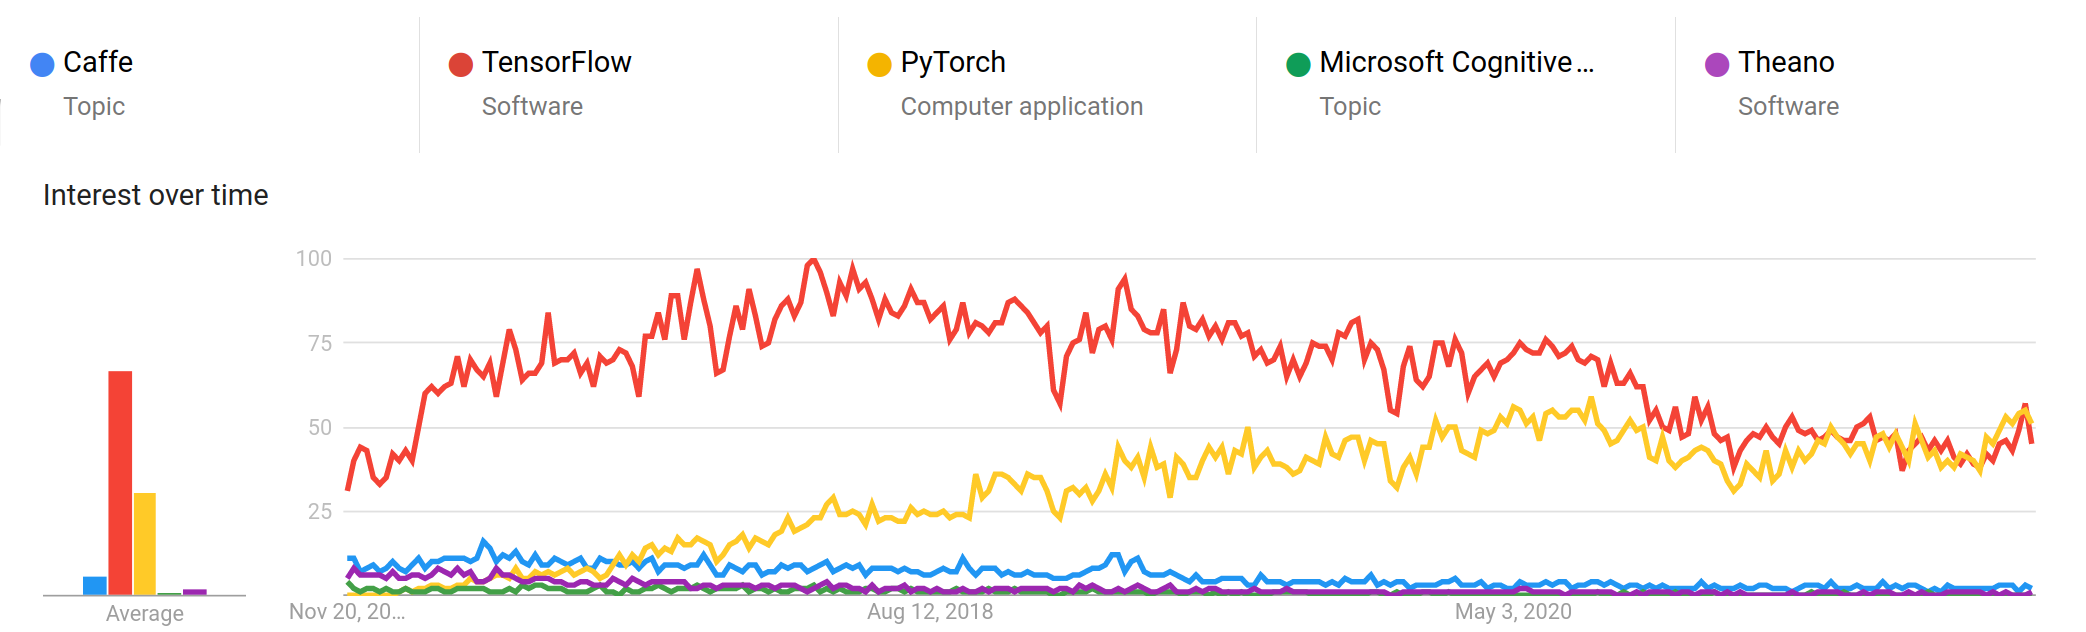
\includegraphics[width=\linewidth]{library_trends.png}
    \caption{Trends for web searches for five of the most popular deep learning frameworks, over the last 5 years.}
    \label{fig:trends}
\end{figure*}

\subsection{About Tensorflow}

- whodunnit
- main features
- small AE example

\subsection{About Pytorch}

- same